%---------------------------------------------------------------------------------------------------------------%
\section{Fase --- E}
%---------------------------------------------------------------------------------------------------------------%

Nesta última fase, implementou-se a funcionalidade de \emph{reset} da tabela de
número hexadecimais, à custa da receção de um \texttt{set-req} no agente,
enviado por um cliente SNMP, com um valor igual à chave de configuração. De
igual modo, pretende-se que a tabela de números hexadecimais seja atualizada com
os valores do ficheiro de sementes iniciais, sendo que após esta operação
o agente pause $R\times10$ segundos, antes de continuar com as operações de
refrescamento da tabela. 


Para implementar os requisitos, necessitou-se alterar a classe
\texttt{MOScalarFactory}, passando como argumento a instância de \texttt{Agent}
e \texttt{AgentHelper}, e por conseguinte, passar os mesmos argumentos
à instância da classe \texttt{ParamAuthReset}, que corresponde aos escalar da
chave da configuração.  Além disso, adicionou-se à classe \texttt{AgentHelper},
o método \texttt{reset}, um método para calcular o tempo de espera após
a operação de \emph{reset}, e também uma variável de condição associada a um
\emph{lock}, para servir de semáforo e uma \emph{flag} booleana para controlar
esse semáforo. 

Na classe \texttt{ParamAuthReset} também se fizerem algumas alterações. Para
o tratamento específico da receção do pedido de \emph{set-req} reescreveram-se
os métodos \texttt{prepare}, \texttt{commit}, \texttt{undo} e \texttt{cleanup}.
Estes métodos são invocados segundo o princípio 2PC (\emph{Two Phase Commit})
onde os valores recebidos de um \texttt{set-req} são validados no
\texttt{prepare} e alterados no \texttt{commit}. Se o \texttt{commit} falhar
todas as alterações são desfeitas no \texttt{undo} e o \texttt{cleanup} para
remover instâncias de objetos criados no processo.       

Com efeito, a comparação do valor de chave do pedido recebida foi implementada no método
\texttt{prepare}, obtendo-se a chave de configuração da instância de
\texttt{AgentHelper}, e aí são comparados os dois valores. Se os valores forem
diferentes, coloca-se o valor do estado do pedido como valor errado, sendo
depois tratado pelo método \texttt{commit}, \texttt{undo} e \texttt{cleanup},
nesta ordem. Note-se que se utilizaram as implementações dos métodos na
super-classe de \texttt{ParamAuthReset}, sendo adicionadas as funcionalidades
pretendidas após essa validação. Assim, quando o método \texttt{commit}
é invocado, se o valor do estado do pedido for igual ao código de valor errado,
o \texttt{commit} falha passando para o \texttt{undo}. Caso o valor do estado
for 0 (sucesso), é executado o que está no corpo do \texttt{commit}, ou seja um
\texttt{Runnable} (processo independente) que executa o método \texttt{reset} do
\texttt{AgentHelper}.  


Na classe \texttt{AgentHelper} modificou-se o método de refrescamento para
implementar o \emph{lock} da variável de condição, enquanto o valor da
\emph{flag} for verdadeira, sendo esta modificada pelo método \texttt{reset}. No
método \texttt{reset} da mesma classe, o algoritmo é o seguinte: quando o método
é invocado, a \emph{flag} é alterada para um valor verdadeiro, seguindo
o carregamento do ficheiro de sementes inicial, remoção do registo da tabela do
agente e criação e registo da nova tabela (conforme a sequência que está no
método \texttt{main} da fase C). Adicionalmente, coloca-se a \emph{flag}
a falso, e calcula-se e guarda-se novamente o tempo de espera, e por fim
sinalizámos o processo que tem o \emph{lock} da variável de condição para
proceder o seu normal funcionamento. 

No método \texttt{main}, no ciclo onde é feito o refrescamento, pausa-se
o processo durante o tempo de espera calculado, e após o o refrescamento da
tabela, alterámos o valor para 0. 

Considere-se também, que o \texttt{set-req} é assíncrono, e, durante uma
operação de refrescamento, o \emph{reset} pode ser despoletado. Neste caso ao
remover a tabela do registo, os valores que estão a ser obtidos no refrescamento
serão nulos. Para evitar uma exceção, colocou-se uma verificação na obtenção de
valores no método de refrescamento, onde caso um valor que seja obtido seja
nulo, o método termina imediatamente, deixando o método de \texttt{reset}
preencher a tabela.  




\subsection{Testes}

\begin{center}
 	
 	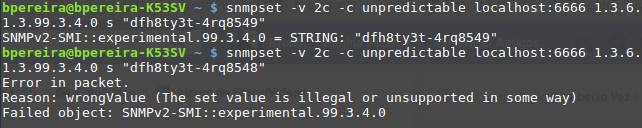
\includegraphics[width=\textwidth,height=\textheight,keepaspectratio]{resources/images/faseE/faseE.png}
 	\captionsetup{type=figure, width=0.8\linewidth}
	\caption{Testes}
\label{fig:faseB:teste} 
\end{center}



